\documentclass{tufte-handout}

%\geometry{showframe}% for debugging purposes -- displays the margins

\usepackage{amsmath}

% Set up the images/graphics package
\usepackage{graphicx}
\setkeys{Gin}{width=\linewidth,totalheight=\textheight,keepaspectratio}
\graphicspath{{graphics/}}

\title{Graduation Gown Care and Etiquette}
\author[Texas Tech University Graduate Student Advsory Council]{Texas Tech University Graduate Student Advsory Council}
\date{}  % if the \date{} command is left out, the current date will be used

% The following package makes prettier tables.  We're all about the bling!
\usepackage{booktabs}

% The units package provides nice, non-stacked fractions and better spacing
% for units.
\usepackage{units}

% The fancyvrb package lets us customize the formatting of verbatim
% environments.  We use a slightly smaller font.
\usepackage{fancyvrb}
\fvset{fontsize=\normalsize}

% Small sections of multiple columns
\usepackage{multicol}

% Provides paragraphs of dummy text
\usepackage{lipsum}

% These commands are used to pretty-print LaTeX commands
\newcommand{\doccmd}[1]{\texttt{\textbackslash#1}}% command name -- adds backslash automatically
\newcommand{\docopt}[1]{\ensuremath{\langle}\textrm{\textit{#1}}\ensuremath{\rangle}}% optional command argument
\newcommand{\docarg}[1]{\textrm{\textit{#1}}}% (required) command argument
\newenvironment{docspec}{\begin{quote}\noindent}{\end{quote}}% command specification environment
\newcommand{\docenv}[1]{\textsf{#1}}% environment name
\newcommand{\docpkg}[1]{\texttt{#1}}% package name
\newcommand{\doccls}[1]{\texttt{#1}}% document class name
\newcommand{\docclsopt}[1]{\texttt{#1}}% document class option name

\makeatletter
\renewcommand{\fnum@figure}{\thefigure}
\makeatother

\begin{document}
\enlargethispage{\baselineskip}

\maketitle% this prints the handout title, author, and date

\marginnote[-1.5\baselineskip]{gsac@ttu.edu}
\marginnote[-0.5\baselineskip]{www.gsac.ttu.edu}

\begin{abstract}
\noindent The fact that you are graduating with your Masters or Doctoral degree is a big deal and means that you have done things right! Now we are here to help you survive the graduation ceremony... mostly by helping you wear you gown, mortar, tassel, and the hood the right way!
\end{abstract}

%\printclassoptions
\noindent In this brief guide we will tell you about caring for your graduation gown, about the graduation etiquette, and a little bit about our gown donation program. If at the end of the graduating ceremony you see us holding ``Gown Donations'' sign please consider donating any regalia that you no longer need. Those gowns will help future generation of Grad Red Raiders.

\begin{marginfigure}[-16\baselineskip]%
\hspace*{0.02in}
  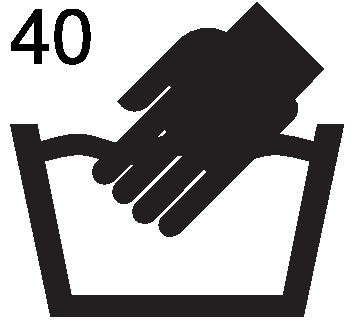
\includegraphics[width=.35\linewidth]{hand-40C}
  \caption{\linespread{1.3}\selectfont{}Hand wash or \hspace{\textwidth}machine wash normal cycle \hspace{\textwidth}$105\,^{\circ}\mathrm{F}$ ($40\,^{\circ}\mathrm{C}$)}
  \label{fig:40C}
\end{marginfigure}

\section{Caring For Your Gown}\label{sec:page-layout}

\subsection{The ``natural way''}
Remove the gown and place on a hanger to allow the folds to fall out, and hang your gown in a high humidity area. A bathroom after a hot shower may be good location.

\begin{marginfigure}[-18\baselineskip]%
\hspace*{0.02in}
  
\includegraphics[width=.35\linewidth]{40C}
  \caption{\linespread{1.3}\selectfont{}Hand wash or \hspace{\textwidth}machine wash normal cycle \hspace{\textwidth}$105\,^{\circ}\mathrm{F}$ ($40\,^{\circ}\mathrm{C}$)}
  \label{fig:40C}
\end{marginfigure}

\subsection{The ``steamy way''}
Consider steaming your gown to remove any wrinkles and freshen it up. Please note that all gowns that the Graduate Student Advisory Council rents out have been previously steam-cleaned.

\begin{marginfigure}[-18\baselineskip]%
\hspace*{0.01in}
  
\includegraphics[width=.35\linewidth]{no-bleach}
  \caption{Do not bleach}
  \label{fig:bleach}
\end{marginfigure}

\subsection{The ``not recommended way''}
\marginnote{Please note that many doctoral gowns should not be ironed. They can only be dry cleaned or steamed. Always follow cleaning instructions provided with your gown.}
If you wish to press your gown, turn it inside out and press with a warm, but \underline{not hot} iron. Always iron exclusive of any decoration a gown may have. 

\begin{marginfigure}[-22\baselineskip]%
\hspace*{0.02in}
  
\includegraphics[width=.35\linewidth]{low-heat-iron}
  \caption{Low heat iron inside out}
  \label{fig:iron}
\end{marginfigure}

\subsection{The ``I am really busy way \#1''}
Your friendly neighborhood dry cleaner can steam the gown for you. Please note that it may be expensive, we would say about \$10.

\begin{marginfigure}[-2\baselineskip]%
\hspace*{0.07in}
  
\includegraphics[width=.30\linewidth]{dry-clean}
  \caption{Dry clean if desiredl}
  \label{fig:dry-clean}
\end{marginfigure}

\subsection{The ``I am really busy way \#2''}
If you are considering dry cleaning your gown you may want to ask your dry-cleaner to use ``green'' cleaning agents. Some of the traditional dry-cleaning chemicals have been linked to cancer. Odds are that smaller neighborhood dry cleaners may not be using eco-friendly cleaners unless specifically requested.

\begin{marginfigure}[-7\baselineskip]%
\hspace*{0.01in}
  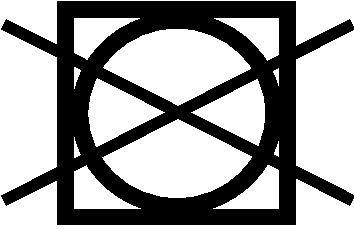
\includegraphics[width=.40\linewidth]{do-not-tumble}
  \caption{Do not tumble dry}
  \label{fig:tumble-dry}
\end{marginfigure}

\newpage
%
%
% NEW PAGE
%
%

\section{Wearing Your Regalia}\label{sec:page-layout}

\begin{marginfigure}[\baselineskip]%
  
\includegraphics[width=.4\linewidth]{gownbw}
  \caption{\linespread{1.3}\selectfont{}Graduation gown}
  \label{fig:gown}
\end{marginfigure}

\subsection{Gown}
In order to look sharp for those pictures that will haunt you for years to come make sure to prepare your gown the day before. We recommending steaming it or dry-cleaning it to remove any wrinkles. A well-fit gown will end midway between the knee and ankle.

\subsection{Hood}
%\marginnote[.5\baselineskip]{Putting a hood can be tricky but don't worry, we will have someone on the floor of the practice hall who will help you make it right!}
The hood should be worn draped around your neck with the largest portion of the hood hanging down your back. The velvet border, which indicates your specific field of study, should be showing on the outside. The velvet should fold under on the lower back to allow the colors of your College or University to show. To keep your hood from being too tight against your neck, there is a cord on the front to help secure it to a shirt button, or pin to a blouse or dress. Many hoods also have a cord and button in the back to prevent your hood from slipping off of your shoulders.

\begin{marginfigure}[-12\baselineskip]%
  
\includegraphics[width=.5\linewidth]{red-cross}
  \caption{\linespread{1.3}\selectfont{}Putting a hood can be tricky but don't worry, we will have someone on the floor of the practice court who will help you make it right!}
  \label{fig:help}
\end{marginfigure}

\subsection{Mortarboard (fancy way of saying a graduation cap!)}
Contrary to common belief your graduation cap should be worn flat on your head and not tilted on the back of your head. The front of the cap should be marked on the inside of your cap.
While men are expected to remove their caps during the school song and the National Anthem, women can keep their caps on.

\begin{marginfigure}[-10\baselineskip]%
  
\includegraphics[width=.5\linewidth]{cap-flat}
  \caption{\linespread{1.3}\selectfont{}Wear your graduation cap flat on your head.}
  \label{fig:flat}
\end{marginfigure}

\subsection{Tassel}

\begin{marginfigure}[\baselineskip]%
\hspace*{0.02in}
  
\includegraphics[width=.45\linewidth]{capbwR}
  \caption{\linespread{1.3}\selectfont{}Tassel worn to the right before your degree is conferred}
  \label{fig:cap-right}
\end{marginfigure}

Tassels are usually worn on the right side and shifted to the left at the end of the graduation ceremony when your degree is officially conferred. Graduation speaker will generally tell you when it is okay to shift your tassel from right to left.

\begin{marginfigure}[\baselineskip]%
\hspace*{0.02in}
  
\includegraphics[width=.45\linewidth]{capbwL}
  \caption{\linespread{1.3}\selectfont{}Tassel worn to the left after your degree is conferred}
  \label{fig:cap-left}
\end{marginfigure}

\section{Dress Code}
In dressing for the graduation it is important to balance dress requirements and comfort. The guiding principle is that your clothing is either covered by the gown, blends in with the gown, or is in harmony with the gown. We recommend at least a business casual dress but also ask that you dress to minimize discomfort. Remember you will not only sit, stand, and walk during the graduation ceremony itself, but also for about two hours during the practice phase. 

\subsection{Women Dress Code}
We recommend wearing dark bottoms: slacks, dress, or skirt, and a light-colored top: dress blouse or dress shirt. 
If you decide to wear a dress we recommend more lightweight choices so the dress does not interfere with shape of the gown. Dresses and skirts should also be shorter than the gown.

We recommend wearing dark shoes: flats or pumps. High heels are not recommended out of concern for your safety and comfort. Sandals and tennis shoes should be avoided. Please make sure not to bring anything with you that will not fit in your pockets. Purses will not be allowed in the graduation court.

\begin{marginfigure}[-12\baselineskip]%
\hspace*{0.02in}
  
\includegraphics[width=.5\linewidth]{bag}
  \caption{\linespread{1.3}\selectfont{}No purses, bags, or backpacks are allowed in the graduation court.}
  \label{fig:bag}
\end{marginfigure}

\subsection{Men Dress Code}
We recommend wearing dark bottoms: trousers or khakis and ironed or pressed light-colored dress shirt with a dark tie. We recommend wearing dark dress shoes and dark socks. Jeans, shorts, sandals and tennis shoes should be avoided.

\begin{marginfigure}[-4\baselineskip]%
\hspace*{0.02in}
  
\includegraphics[width=.5\linewidth]{backpack}
  \caption{\linespread{1.3}\selectfont{}No backpacks are allowed in the graduation court.}
  \label{fig:bag}
\end{marginfigure}

\vspace*{.2\baselineskip} % inserts empty line

\section{Returning or Donating Your Regalia}
We will be present after at the graduation arena and you will be able to return or donate your regalia to us as you are walking out and for another hour.  Alternatively, you can return or donate your gown the following week by dropping it off by the Graduate School in the Administration Building room 328. It is the third floor of the east wing of the administration building.

\marginnote{\textbf{Drop-off Address:}\hspace{\textwidth}
Texas Tech University\hspace{\textwidth}
Graduate School\hspace{\textwidth}
Administration Building. Room 328\hspace{\textwidth}
(3rd Floor, East Wing)\hspace{\textwidth}
Lubbock, TX 79409-1030\hspace{\textwidth}
\newline
~\\
\noindent\textbf{Postal address:}\hspace{\textwidth}
Graduate Student Advisory Council\hspace{\textwidth}
Texas Tech University\hspace{\textwidth}
Mail Stop 1030\hspace{\textwidth}
Lubbock, TX 79409-1030\hspace{\textwidth}
\newline
~\\
\noindent \textbf{Courier delivery (FedEx, UPS):}\newline
\noindent Texas Tech GSAC\newline
\noindent Boston Ave. at Akron Ave.\newline
\noindent Administration Bldg. Room 328\newline
\noindent Lubbock, TX 79409-1030\newline
}
~\\
\noindent The free graduation gown rental program is only possible due to generous donations from graduate students like you!!! We make donating gowns as easy and as painless as possible and offer several flexible donation options:

\begin{description}
\item[On-site] We will be present at the graduation. You can leave your  gown with us after the ceremony!
\item[Pick-up] If you send us an email to gsac@ttu.edu we will be glad to pick up the gown from any Lubbock location!
\item[Drop-off] Regalia can be donated at the front desk in the Graduate School, Administration Building, room 328.
\item[Mail-in] If you are based outside of Lubbock please fell free to mail your gown to us. If you would like to we can email you a prepaid shipping label. Simply send us an email to gsac@ttu.edu.
\end{description}

\begin{fullwidth}
\Huge{\textit{Congratulations and Thank You!!!}}
\end{fullwidth}


The gown for the master's degree has an oblong sleeve, open at the wrist, like the others. The sleeve base hangs down in the traditional manner. The rear part of its oblong shape is square cut, and the front part has an arc cut away. The gown is so designed and supplied with fasteners that it may be worn open or closed. The gown for the doctor's degree has bell-shaped sleeves. It is so designed and supplied with fasteners that it may be worn open or closed.
master's degrees are untrimmed. For the doctor's degree, the gown is faced down the front with black velvet; three bars of velvet are used across the sleeves. These facings and crossbars may be of velvet of the color distinctive of the disciplines to which the degree pertains, thus agreeing in color with the binding or edging of the hood appropriate to the particular doctor's degree in every instance.

For all academic purposes, including trimmings of doctors' gowns, edging of hoods, and tassels of caps, the colors associated with the different disciplines are as follows: 

\begin{margintable}
\begin{tabular}{ll}
Agriculture                     & Maize         \\
Arts and Humanities             & White         \\
Business                           & Drab          \\
Economics                       & Copper        \\
Education                       & Light Blue    \\
Engineering                     & Orange        \\
Fine Arts                       & Brown         \\
Architecture                    & Brown         \\
Journalism                      & Crimson       \\
Music                           & Pink          \\
Philosophy                      & Dark Blue     \\
Physical Education              & Sage Green    \\
Public Administration           & Peacock Blue  \\
Science                         & Golden Yellow \\
Social Work                     & Citron       
\end{tabular}
\end{margintable}


Hoods

Pattern
As usually followed by American colleges and universities, but following the specifications listed below.

Material
In all cases the material must be the same as that of the gown.
 
Color
Black in all cases.
 
Length
The length of the hood worn for the bachelor's degree must be three feet, for the master's degree three and one-half feet, and for the doctor's degree, four feet. The hood worn for the doctor's degree only shall have panels at the sides.
 
Linings
The hoods are to be lined with the official color or colors of the college or university conferring the degree; more than one color is shown by division of the field color in a variety of ways, chevron or chevrons, equal division, etc. The various academic costume companies maintain complete files on the approved colors for various institutions.
 
Trimmings
The binding or edging of the hood is to be velvet or velveteen, two inches, three inches, and five inches wide for the bachelor's, master's, and doctor's degrees, respectively; the color should be indicative of the subject to which the degree pertains (see above). For example, the trimming for the degree of Master of Science in Agriculture should be maize, representing agriculture, rather than golden yellow, representing science. No academic hood should ever have its border divided to represent more than a single degree.

In the case of the Doctor of Philosophy degree, the dark blue color is used to represent the mastery of the discipline of learning and scholarship in any field that is attested to by the awarding of this degree and is not intended to represent the field of philosophy.


The custom of wearing academic gowns, hoods, and caps dates back to about the 12th century, when most scholars belonged to a religious order.

Long gowns and hoods were standard dress for medieval clergy, who often studied and taught in cold buildings. The style and coloring of the robe, hood, and, sometimes, skull cap denoted an edu­cated individual. From the end of the 16th century to the present, members of the clergy, law profes­sionals, and academics have worn robes.

Sometime in the 14th century, English univer­sities began to use the dress to distinguish levels of education. Modeled on the English system, the American Academic Costume Code was estab­lished in 1895 by a commission of delegates from the Ivy League and New York universities.

The Costume Code calls for three types of gowns: doctoral, master’s, and bachelor’s. The doc­toral gown is the most elaborate, with front-facing velvet and three velvet bars on each of the full, bil­lowing sleeves. The velvet can be black, PhD blue, or the academic color to which the degree corre­sponds. The master’s gown is distinctive for its ex­tremely long, closed sleeves, the arms protruding through a slit at the elbow. The bachelor’s gown is the simplest of the three, a plain gown with long, pointed sleeves.

Doctoral and master’s degrees are also indicat­ed by a hood, distinctive in shape, size, and color. The doctor’s hood is easily recognizable, with wide velvet edging that indicates the degree earned and full exposure of the lining. The master’s hood is the same length as the doctor’s hood but does not fully expose the lining, and the velvet edging is not as wide. For both hoods, the lining indicates the col­ors of the institution conferring the degree.

Mortarboards, the distinctive four-pointed caps, are worn by academics at all levels. In recent years, doctors have taken to wearing a soft velvet tam instead.

\end{document}
